\subsection{Completed Runs and Initial Performance}
All 24 specified branches completed the fixed budget. Separate readback verified 432 evaluation episodes and 48 saved candidate checkpoints, with the six original source checkpoints unchanged. Paired replay variants produced identical initial evaluation returns. The complete study, including clean replay collection, evaluation, checkpoint writing, and initialization, took 1,463.8 seconds on the recorded machine. Table~\ref{tab:outcomes} gives the equally weighted mean over the three source seeds; returns are environment reward sums, not completion rates.

\begin{table}[t]
\caption{Fixed-budget pilot outcomes, averaged equally across three source seeds. $B(0)$ and $B(4000)$ are new-condition returns before and after adaptation; $\Delta A$ is the old clean-condition return change. Returns are not success percentages.}
\label{tab:outcomes}
\centering\small
\begin{tabular*}{\textwidth}{@{\extracolsep{\fill}}llrrrr@{}}
\toprule
Controller & Fault & $\rho$ & $B(0)$ & $B(4000)$ & $\Delta A$ \\
\midrule
Transformer & Noise & 0 & 2433.7 & 2130.1 & $-320.9$ \\
Transformer & Noise & 0.5 & 2433.7 & 2105.1 & $-272.4$ \\
Transformer & Delay & 0 & -85.5 & 12.6 & $-825.4$ \\
Transformer & Delay & 0.5 & -85.5 & -75.3 & $-145.2$ \\
Reactive & Noise & 0 & 2875.5 & 2369.7 & $-641.2$ \\
Reactive & Noise & 0.5 & 2875.5 & 2727.3 & $-339.0$ \\
Reactive & Delay & 0 & -180.3 & 203.4 & $-1158.9$ \\
Reactive & Delay & 0.5 & -180.3 & 47.9 & $-383.9$ \\
\bottomrule
\end{tabular*}
\end{table}


The initial clean-condition means were 2,677.9 (transformer) and 3,328.1 (reactive). The zero-step sensor conditions differed substantially. Mean noise-condition return was 2,433.7 for the transformer and 2,875.5 for the reactive controller. Under the three-step delay, the corresponding means were $-85.5$ and $-180.3$. These are measurements after applying the sensor intervention and before continued training. Different initial performance and source-policy quality constrain cross-controller interpretation.

\subsection{Adaptation under Noise and Delay}
Figure~\ref{fig:adaptation} shows the fixed-budget learning curves. Under noise, mean return declined for both controllers with either replay strategy. Transformer return changed by $-303.7$ without retained replay and $-328.7$ with it. Reactive return changed by $-505.8$ and $-148.2$, respectively. Thus, continued training did not yield a mean noise-condition improvement within this budget, even though the reactive retained-replay arm declined less.

\begin{figure}[!htbp]
\centering
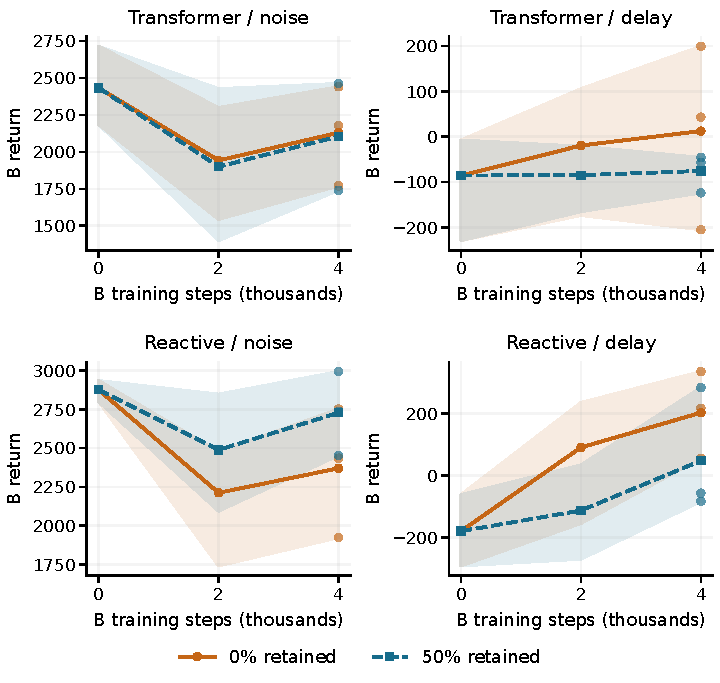
\includegraphics[width=\textwidth]{sensor_adaptation.pdf}
\caption{New-condition return during continued training. Lines are means over three source seeds; shaded bands are their minimum--maximum ranges, not confidence intervals. Small points at the final budget show individual seed means. Evaluation uses three deterministic episodes per seed and condition.}
\label{fig:adaptation}
\end{figure}

Delay produced positive mean changes but substantial variation. Without retained replay, the transformer gained 98.1 return units and the reactive controller gained 383.7. With retained replay, the corresponding gains were 10.2 and 228.2. The transformer's no-replay seed-level changes ranged from $-197.9$ to $+428.8$; its retained-replay changes ranged from $-38.4$ to $+105.4$. Only two of three transformer seeds improved without replay, and one of three improved with replay. All three reactive seeds improved under delay in both replay variants. These counts describe this pilot's realized seed outcomes, not estimated population success probabilities.

The trapezoidal mean return across the sampled learning curve was $-27.8$ without replay and $-82.6$ with replay for transformer delay, compared with 51.2 and $-89.8$ for reactive delay. This summary includes intermediate deterioration that a final-point comparison would hide. It does not establish a recovery time because no recovery threshold was specified.

\subsection{Retention and Paired Replay Effects}
Every branch had a negative clean-condition change at the final budget (Fig.~\ref{fig:retention}). For transformer delay, the mean loss was 825.4 without retained replay and 145.2 with replay. For reactive delay, it was 1,158.9 and 383.9. The corresponding noise-condition adaptation branches lost 320.9 versus 272.4 for the transformer and 641.2 versus 339.0 for the reactive controller.

\begin{figure}[!htbp]
\centering
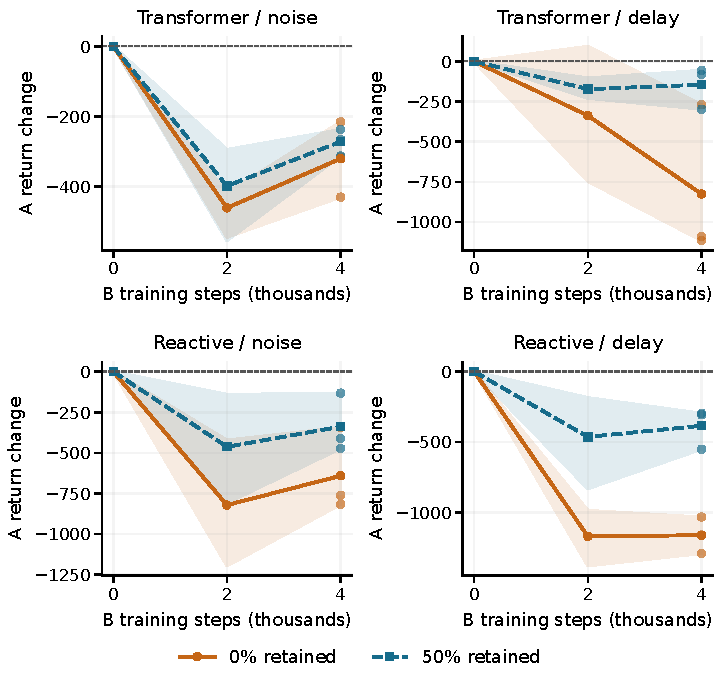
\includegraphics[width=\textwidth]{sensor_retention.pdf}
\caption{Clean-condition retention measured with the actual updated model. Zero is each branch's own initial clean-condition return. Negative values indicate loss of earlier measured performance. Lines and shaded ranges summarize three source seeds; the ranges are not confidence intervals.}
\label{fig:retention}
\end{figure}

Retained replay increased final clean-condition return relative to the paired no-replay branch in ten of twelve seed/controller/fault pairs. Its mean effect on clean return was positive in all four controller/fault comparisons. This was not uniform at the seed level: transformer seed 43 under noise and seed 42 under delay retained less with replay. For both controllers, all three delay seeds ended with lower delay-condition return under retained replay than under no replay. The paired comparison therefore exposes a cost in new-condition performance alongside improved average retention under delay. Neither arm preserved its own initial clean performance.

Mean collection-and-optimization time per branch ranged from 55.1 to 75.0 seconds across transformer conditions and from 34.9 to 38.3 seconds across reactive conditions. Those times exclude evaluation and checkpoint I/O. They describe this implementation and machine load; they do not establish equal computational budgets or a generally faster adaptation algorithm.
